\documentclass[12pt, twoside]{article}
\usepackage[letterpaper, margin=1in, headsep=0.5in]{geometry}
\usepackage[english]{babel}
\usepackage[utf8]{inputenc}
\usepackage{amsmath}
\usepackage{amsfonts}
\usepackage{amssymb}
\usepackage{tikz}
%\usetikzlibrary{quotes, angles}

\usepackage{graphicx}
\usepackage{enumitem}
\usepackage{multicol}

\usepackage{fancyhdr}
\pagestyle{fancy}
\fancyhf{}
\renewcommand{\headrulewidth}{0pt} % disable the underline of the header

\fancyhead[LE]{\thepage}
\fancyhead[RO]{\thepage \\ Name: \hspace{4cm} \,\\}
\fancyhead[LO]{BECA / Dr. Huson / Geometry\\* Unit 6: Distance \& slope\\* 10 December 2019}

\begin{document}
\subsubsection*{6.10b Classwork: Dilation and similarity\\[0.25cm]
(complete 12 stars per group)}
  \begin{enumerate}
  
  \item A dilation centered at $A$ maps $\triangle ABC \rightarrow \triangle ADE$. Given the sides of the preimage, $AC = 4$, $BC = 3$, $AB = 5$, and of $DE = 6$ find the scale factor $k$ and the lengths $AD$ and $AE$. Then find $CE$ and $BD$. \hfill (1 star each value. 5 stars total)
    \begin{flushright}
      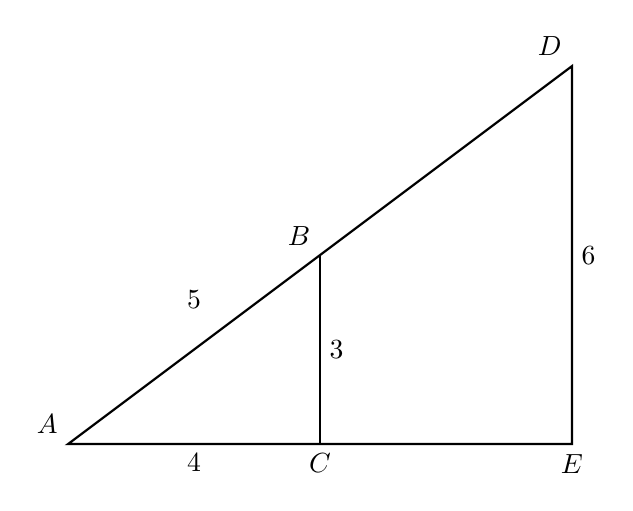
\begin{tikzpicture}[scale=0.8]
        \draw [-, thick] (0,0) node[above left]{$A$}--
        (8,0) node[below]{$E$}--
        (8,6) node[above left]{$D$}--cycle;
        \draw [thick] (4,0)--(4,3);
        \node at (4,0) [below]{$C$};
        \node at (4,3) [above left]{$B$};
        \node at (2, 0) [below]{$4$};
        \node at (2, 2) [above]{$5$};
        \node at (8, 3) [right]{$6$};
        \node at (4, 1.5) [right]{$3$};
      \end{tikzpicture}
    \end{flushright} \vspace{1.5cm}
  
  \item Triangle $ABC$ is dilated with a scale factor of $k$ centered at $A$, yielding $\triangle ADE$, as shown. Given $AB=8$, $BC=12$, $AC=16$, and $DE=18$. \\[0.25cm] Find the scale factor $k$ and the segment lengths $AD$ and $CE$. \hfill (2 stars each. 6 total)
    \begin{flushright}
      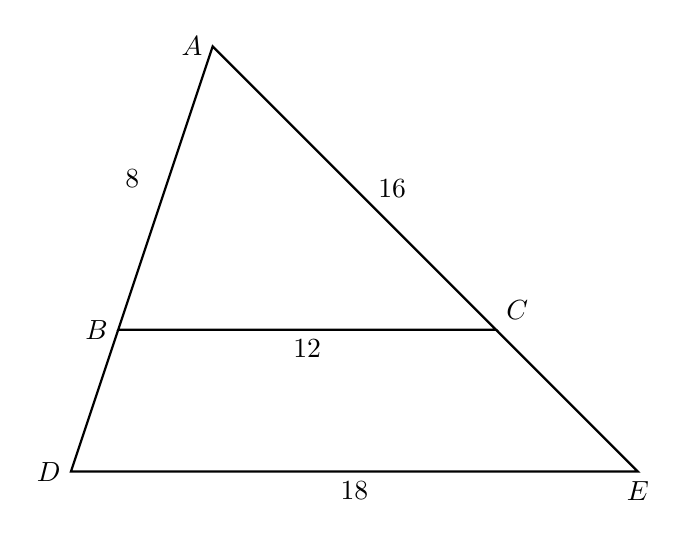
\begin{tikzpicture}[scale=0.6]
        \draw [thick]
        (0,0)node[left]{$B$}--
        (8,0)node[above right]{$C$}--
        (2,6)node[left]{$A$}--cycle;
        \draw [thick]
        (0,0)--
        (-1,-3)node[left]{$D$}--
        (11,-3)node[below]{$E$}--(8,0);
        \node at (4,0)[below]{$12$};
        \node at (5.3, 3)[right]{$16$};
        \node at (0.3, 2.8)[above]{$8$};
        \node at (5,-3)[below]{$18$};
      \end{tikzpicture}
    \end{flushright} \vspace{2.5cm}

\newpage
  \item A dilation maps triangle $KLM$ onto triangle $PQR$, with $KM=3$, $LM=3.3$, $PR=5$. \vspace{0.5cm}
    \begin{multicols}{2}
    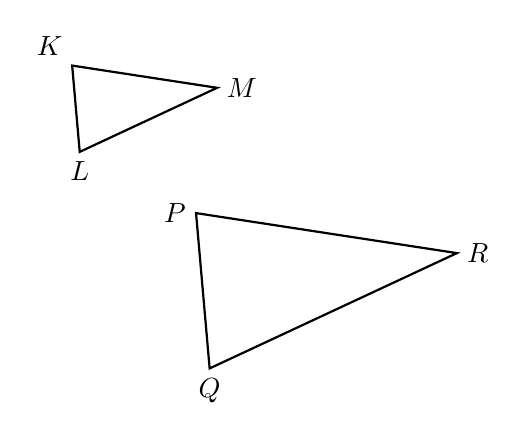
\begin{tikzpicture}[scale=0.55]
      \coordinate [label=above left:$K$](A) at (95:2);
      \coordinate [label=below:$L$](B) at (0, 0);
      \coordinate [label=right:$M$](C) at (25:3.5);
      \draw [thick] (A)--(B)--(C)--cycle;

      \draw [thick, xshift=3cm, yshift=-5cm, scale=1.8] (95:2) node[left]{$P$}--
      (0,0) node[below]{$Q$}--
      (25:3.5) node[right]{$R$}--cycle;
    \end{tikzpicture}\\
    Write each corresponding object.
    \begin{enumerate}
      \item $L \rightarrow$ \rule{2cm}{0.15mm} \hfill (1 star)
      \item $\angle K \cong$ \rule{2cm}{0.15mm} \hfill (1 star)
      \item $QR=$ \rule{2cm}{0.15mm}  \hfill (1 star)
      \item Justify $\triangle KLM \sim \triangle PQR$. Use the words ``maintains angles" and ``dilation''. \qquad \qquad (2 stars)
    \end{enumerate}
  \end{multicols} \vspace{2cm}

  \item Given $\triangle ABC \sim \triangle DEF$. $m\angle A = 45^\circ$ and $m\angle E = 50^\circ$. Find the measure of $\angle F$. \\ (3 stars)\vspace{3cm}

  \item Given $\triangle ABP \sim \triangle JKP$ as shown below. $AB=9.6$, $AP=12.0$, $BP=6.3$, and $JK=16.0$. Find $JP$. \hfill (3 stars)
    \begin{flushright}
    \begin{tikzpicture}[scale=1.4]
        \draw [thick]
          (-0.25,-1)node[below left]{$B$}--
          (0.5,2)node[left]{$K$}--
          (4,0)node[below left]{$J$}--
          (0,0)node[above left]{$P$}--
          (-2,0)node[left]{$A$}--cycle;
      \end{tikzpicture}
      \end{flushright}
      \vspace{2cm}

\newpage
  \item A rotation of $90^\circ$ is applied to $\triangle ABC$, mapping it onto $\triangle PQR$, as shown.
  Which triangle has the larger area, or are they equal? Justify your answer.\\
      \begin{tikzpicture}[scale=.4]
        \draw [thick, <->] (-7.4,0) -- (10.4,0) node [right] {$x$};
        \draw [thick, <->] (0,-4.4)--(0,10.4) node [above] {$y$}; 
        \draw [thick]
          (4,-2) node[below right] {$A$}--
          (8,2) node[right] {$B$}--
          (2,1) node[left] {$C$}--cycle;
        \draw [thick]
          (2,4) node[right] {$P$}--
          (-2,8) node[above] {$Q$}--
          (-1,2) node[left] {$R$}--cycle;
      \end{tikzpicture}

  \begin{multicols}{2}
    [\item A translation maps triangle $KLM$ onto triangle $PQR$.] \vspace{0.5cm}
      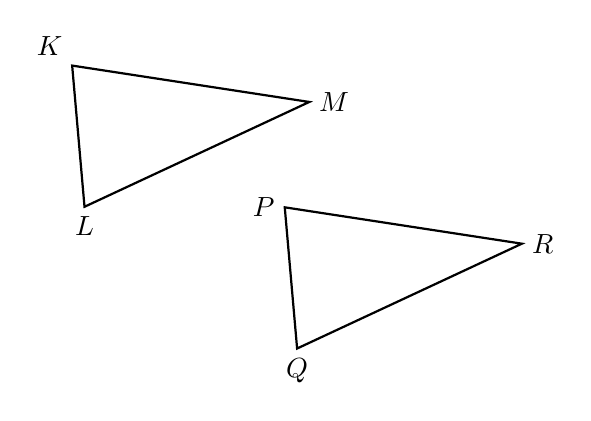
\begin{tikzpicture}[scale=0.9]
        \coordinate [label=above left:$K$](A) at (95:2);
        \coordinate [label=below:$L$](B) at (0, 0);
        \coordinate [label=right:$M$](C) at (25:3.5);
        \draw [thick] (A)--(B)--(C)--cycle;

        \draw [thick, xshift=3cm, yshift=-2cm] (95:2) node[left]{$P$}--
        (0,0) node[below]{$Q$}--
        (25:3.5) node[right]{$R$}--cycle;
      \end{tikzpicture}\\
      Write each corresponding object.
      \begin{enumerate}
        \item $L \rightarrow$ \rule{2cm}{0.15mm}
        \item $\angle M \cong$ \rule{2cm}{0.15mm}
        \item \rule{2cm}{0.15mm} $\cong \overline {QR}$
        \item Justify $\triangle KLM \cong \triangle PQR$. Use the words ``rigid motion" and ``translation''.
      \end{enumerate}
    \end{multicols}  \vspace{1.5cm}
  
  \item Find the image of $P(-4,0)$ after the translation $(x,y) \rightarrow (x-10,y+2)$.    

  \item Translate $\triangle ABC$ by $(x,y) \rightarrow (x+6, y-3)$. Make a table of the coordinates and plot and label the image on the axes.
  \begin{flushright}
    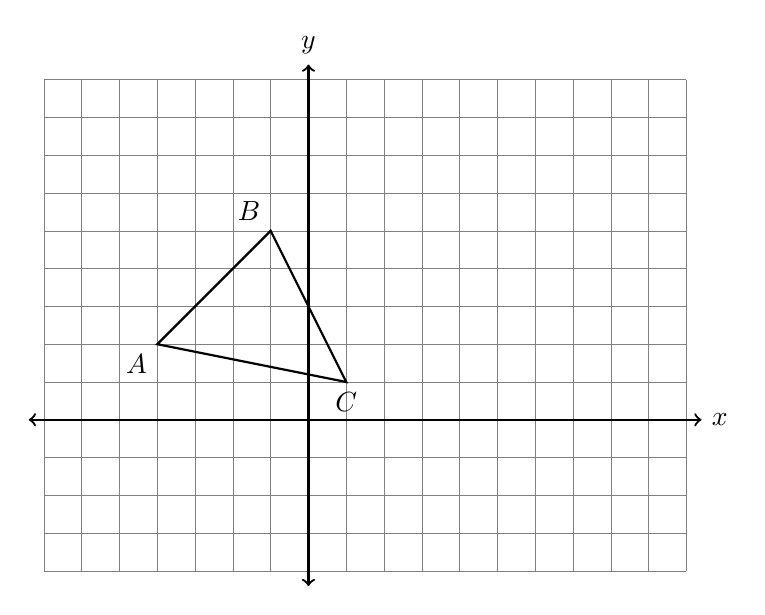
\begin{tikzpicture}[scale=.48]
      \draw [help lines] (-7,-4) grid (10,9);
      \draw [thick, <->] (-7.4,0) -- (10.4,0) node [right] {$x$};
      \draw [thick, <->] (0,-4.4)--(0,9.4) node [above] {$y$};  
      \draw [thick]
        (-4,2) node[below left] {$A$}--
        (-1,5) node[above left] {$B$}--
        (1,1) node[below] {$C$}--cycle;  
  \end{tikzpicture}
  \end{flushright}

\newpage
\item The side $\overline{AB}$ of triangle $ABC$ is extended and an altitude to the vertex $C$ is drawn, as shown below. The triangle's height is $h=4.8$ and its base measures $AB=7.1$. Find the area of the triangle.
\begin{flushright}
  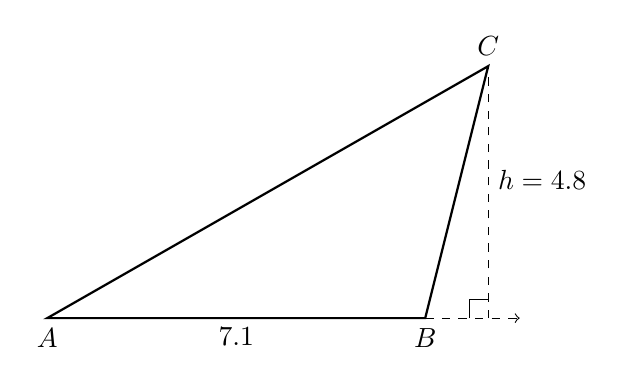
\begin{tikzpicture}[scale=0.8]
    \draw [thick]
      (0,0)node[below]{$A$}--
      (6,0)node[below]{$B$}--
      (7,4)node[above]{$C$} --cycle;
  \draw [dashed] (7,0)--(7,4);
  \draw [dashed, ->] (6,0)--(7.5,0);
  \draw (7,0)++(-0.3,0)--++(0,0.3)--+(0.3,0);
  \node at (7,2.2)[right]{$h=4.8$};
  \node at (3,0)[below]{$7.1$};
  \end{tikzpicture}
\end{flushright}

\item One side of the $\triangle ABC$ has a length $AB=12$. The triangle's area is $45$. Find the length of the altitude $h$ of the triangle to vertex $C$ and perpendicular to side $\overline{AB}$.\\[0.5cm]
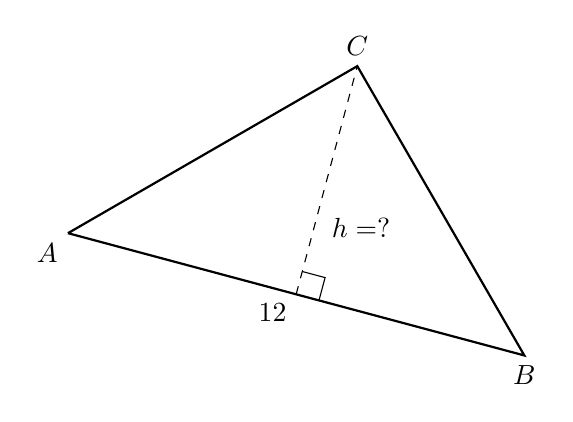
\begin{tikzpicture}[scale=1, rotate=-15]
\draw [thick]
(2,0)node[below left]{$A$}--
(8,0)node[below]{$B$}--
(5,3)node[above]{$C$} --(2,0);
\draw [dashed] (5,0)--(5,3);
\draw (5,0)++(0.3,0)--++(0,0.3)--+(-0.3,0);
\node at (5.1,0.9)[right]{$h=?$};
\node at (5,0)[below left]{$12$};
\end{tikzpicture} \vspace{1.0cm}

\item The point $K$ is the midpoint of $\overline{JL}$, $JK=-x+13$, and $JL=2x-2$. Find ${JK}$.  \vspace{1cm}
\begin{flushright}
  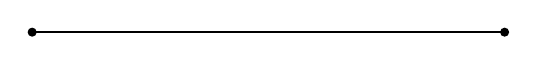
\begin{tikzpicture}
    \draw [-, thick] (0,0)--(6,0);
    \draw [fill] (0,0) circle [radius=0.05];
    \draw [fill] (6,0) circle [radius=0.05];
  \end{tikzpicture}
  \end{flushright} \vspace{2cm}

\newpage
\item Given two parallel lines and a transversal, as shown below.
\begin{center}
\begin{tikzpicture}
  \draw [<->, thick] (1,2)--(9,2);
  \draw [<->, thick] (0,0)--(8,0);
  \draw [<->, thick] (4,-1)--(5.5,3);
  \node at (4.5,0.3) [left]{$5$};
  \node at (4.5,0.3) [right]{$6$};
  \node at (4.3,-0.3) [left]{$7$};
  \node at (4.3,-0.3) [right]{$8$};
  \node at (5.2,2) [above left]{$1$};
  \node at (5.2,2) [above right]{$2$};
  \node at (5,2) [below left]{$3$};
  \node at (5,2) [below right]{$4$};
\end{tikzpicture}
\end{center}
\begin{enumerate}
  \item State the angle corresponding with $\angle 7$. \vspace{0.5cm}
  \item What theorem would justify $m\angle 4 + m\angle 6 =180^\circ$? \rule{5cm}{0.15mm} \vspace{0.5cm}
  \item What theorem would justify $\angle 3 \cong \angle 6$? \rule{7cm}{0.15mm} \vspace{0.5cm}
  \item Given $m\angle 1 = 117^\circ$ and $m\angle 8 = (4x-3)^\circ$. Find $x$. \vspace{3.5cm}
\end{enumerate}

\item A translation maps $X(1,7) \rightarrow X'(-3,9)$. What is the image of $Y(0,-3)$ under the same translation?  \vspace{2cm}

\item Given isosceles $\triangle RSU$ with $\overline{US} \cong \overline{RS}$. If $m\angle UST=150$ find $m\angle U$.
\begin{flushright}
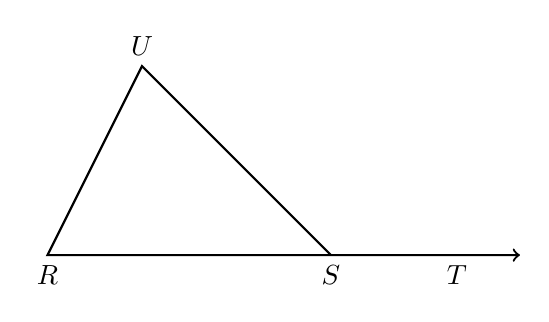
\begin{tikzpicture}[scale=0.8]
  %\draw [->, thick] (0,0)--(5,5);
  \draw [<-, thick] (8,0)--
    (7,0) node[below]{$T$}--
    (0.5,0) node[below]{$R$}--
    (2,3) node[above]{$U$}--
    (5,0) node[below]{$S$};
\end{tikzpicture}
\end{flushright} \vspace{1cm}

\item Given isosceles $\triangle TUV$ with $\overline{TU} \cong \overline{UV}$ and $m\angle T = 55$. Find $m\angle U$ and $m\angle V$.
\begin{flushright}
  (\emph{the diagram is not to scale})\\
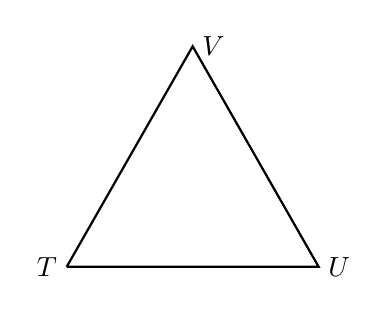
\begin{tikzpicture}[scale=0.8]
  \draw [thick](0,0)--(4,0)--(2,3.5)--(0,0);
  \node at (0,0) [left]{$T$};
  \node at (4,0) [right]{$U$};
  \node at (2,3.5) [right]{$V$};
\end{tikzpicture}
\end{flushright}

\newpage
\item The trapezoid $ABCD$, shown below, undergoes a rigid transformation carrying it onto trapezoid $WXYZ$. State the transformation. (be specific)\\
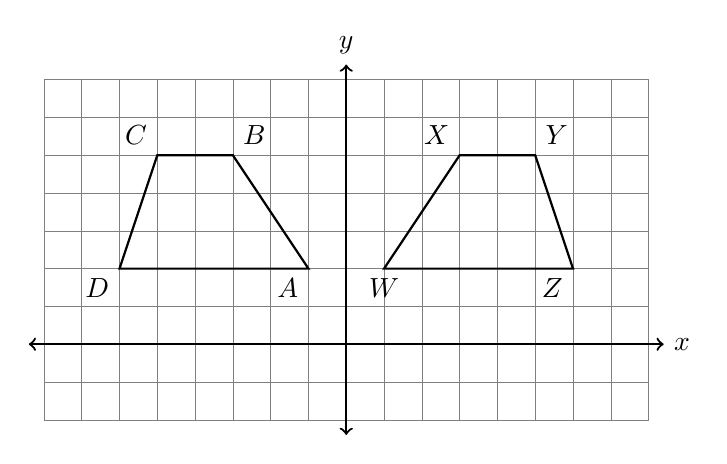
\begin{tikzpicture}[scale=.48]
  \draw [help lines] (-8,-2) grid (8,7);
  \draw [thick, <->] (-8.4,0) -- (8.4,0) node [right] {$x$};
  \draw [thick, <->] (0,-2.4)--(0,7.4) node [above] {$y$};
  \draw [thick]
    (6,2) node[below left] {$Z$}--
    (5,5) node[above right] {$Y$}--
    (3,5) node[above left] {$X$}--
    (1,2) node[below] {$W$}--cycle;
  \draw [thick]
    (-1,2) node[below left] {$A$}--
    (-3,5) node[above right] {$B$}--
    (-5,5) node[above left] {$C$}--
    (-6,2) node[below left] {$D$}--cycle;
\end{tikzpicture}

\item The points $R$, $S$, and $T$ are collinear, with $RS=4x-8$, $ST=21$, and $RT=6x-1$. \\*[0.25cm]
Find ${RT}$. \vspace{0.5cm}
\begin{flushright}
  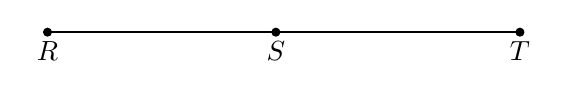
\begin{tikzpicture}
    \draw [-, thick] (0,0)--(6,0);
    \draw [fill] (0,0) circle [radius=0.05] node[below]{$R$};
    \draw [fill] (2.9,0) circle [radius=0.05] node[below]{$S$};
    \draw [fill] (6,0) circle [radius=0.05] node[below]{$T$};
  \end{tikzpicture}
  \end{flushright} \vspace{4cm}

\item In the diagram below, $\triangle ABC$ with sides of 11, 15, and 16, is mapped onto $\triangle DEF$ after a clockwise rotation of $90^\circ$ about point $P$. \\*[0.25cm]
If $DF=2x+1$, what is the value of $x$? 
    \begin{flushright}
      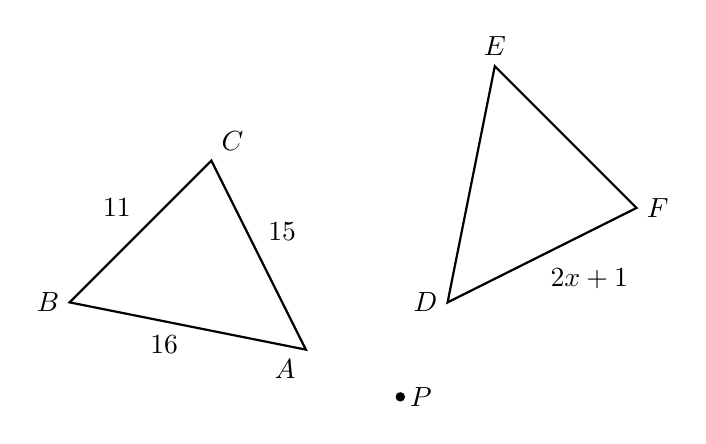
\begin{tikzpicture}[scale=.6]
        %\draw [thick, <->] (-7.4,0) -- (10.4,0) node [right] {$x$};
        %draw [thick, <->] (0,-5.4)--(0,10.4) node [above] {$y$};
        \fill (0,0) circle[radius=0.1] node[right]{$P$};
        \draw [thick]
          (-2,1) node[below left] {$A$}--
          (-7,2) node[left] {$B$}--
          (-4,5) node[above right] {$C$}--cycle;
          \node at (-5,1.5)[below]{16};
          \node at (-6,4){11};
          \node at (-2.5,3.5){15};
          \node at (4,2.5){$2x+1$};
        \draw [thick]
          (1,2) node[left] {$D$}--
          (2,7) node[above] {$E$}--
          (5,4) node[right] {$F$}--cycle;
      \end{tikzpicture}
    \end{flushright}  \vspace{1cm}

\newpage
\item Given $\triangle ABC$ point $D$ on $\overline{AB}$ and point $E$ on $\overline{BC}$ such that $\triangle ABC \sim \triangle DBE$. \\*[0.25cm]
If $AB=15$, $BC=10$, and $AD=9$, what is the length of $\overline{BE}$?
  \begin{flushright}
    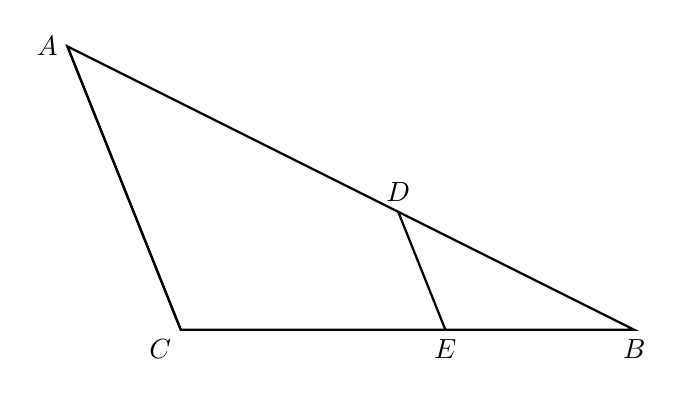
\begin{tikzpicture}[scale=0.6]
      \coordinate [label=left:$A$](A) at (-12,6);
      \coordinate [label=below:$B$](B) at (0, 0);
      \coordinate [label=below left:$C$](C) at (-9.6,0);
      \coordinate [label=above:$D$](D) at (-5, 2.5);
      \coordinate [label=below:$E$](E) at (-4,0);
      \draw [thick] (A)--(B)--(C)--cycle;
      \draw [thick] (A)--(C);
      \draw [thick] (D)--(E);
    \end{tikzpicture}
  \end{flushright} \vspace{3cm}

\item In  $\triangle ABC$ shown below, $m\angle A=(10x)^\circ$, $m\angle B=(16x-5)^\circ$, and $m\angle C=(2x+3)^\circ$. \\[0.25cm] 
Find $m\angle A$. (show the check for full credit)
\begin{flushright}
    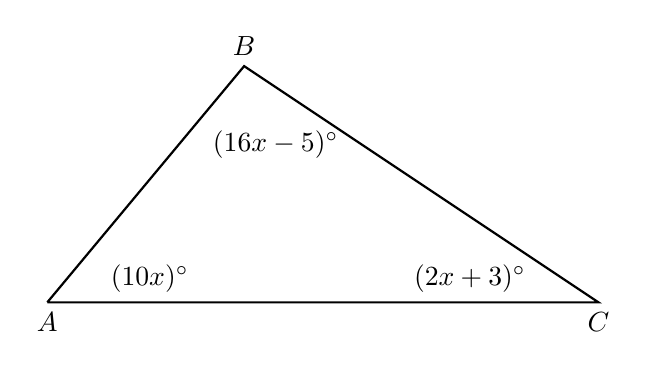
\begin{tikzpicture}
      \draw [thick]
        (2,0)node[below]{$A$}--
        (9,0)node[below]{$C$}--
        (4.5,3)node[above]{$B$} --(2,0);
        \node at (3.3,0)[above]{$(10x)^\circ$};
        \node at (8.2,0)[above left]{$(2x+3)^\circ$};
        \node at (4.9,2.3)[below]{$(16x-5)^\circ$};
    \end{tikzpicture}
  \end{flushright}

\newpage
\item The shape shown below is composed of straight lines and right angles, with some lengths as marked. Find the area of the figure. (the figure is not drawn to scale)
\begin{flushleft}
\begin{tikzpicture}[scale=0.5]
\draw [-, thick] (0,0)--(13,0)--(13,3)--(9,3)--(9,9)--
(0,9)--(0,7)--(4,7)--(4,3)--(0,3)--cycle;
%\draw [fill] (0,0) circle [radius=0.05] node[left]{$A$};
%\draw [fill] (7,0) circle [radius=0.05] node[right]{$B$};
%\draw [fill] (7,2) circle [radius=0.05] node[right]{$C$};
%\draw [fill] (0,2) circle [radius=0.05] node[left]{$D$};
\node at (4.5, 5){4};
\node at (2, 2.5){4};
\node at (8.5, 6){6};
\node at (11, 2.5){4};
\node at (6.5, -0.5){13};
\node at (13.5, 1.5){3};
%\node at (13.5, 8){2};
\end{tikzpicture}
\end{flushleft} \vspace{3cm}

\item $\triangle ABC$ is shown with vertices $A(2,-3)$, $B(6,1)$, and $C(3,4)$. Reflect the triangle across the $x$-axis. Write down its coordinates in a table and plot and label it on the graph.
  \begin{flushright}
    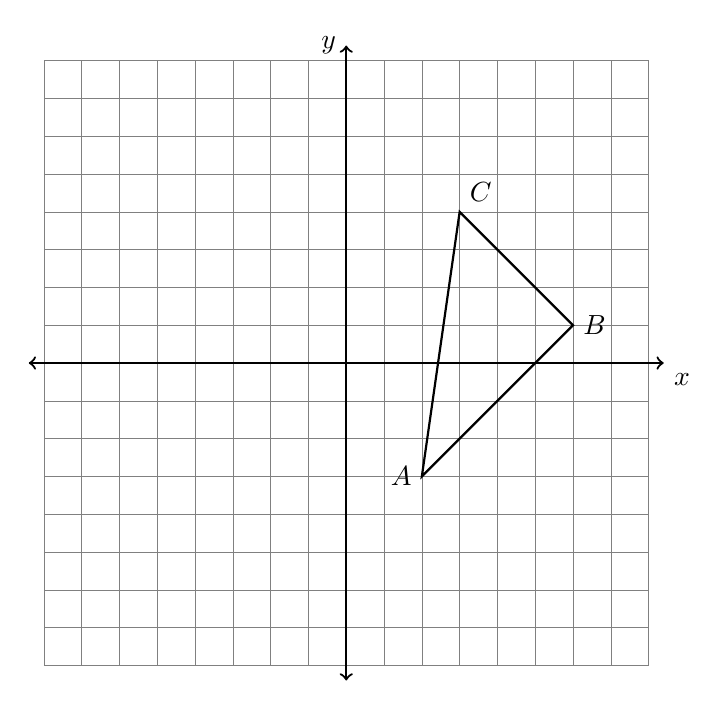
\begin{tikzpicture}[scale=.48]
      \draw [help lines] (-8,-8) grid (8,8);
      \draw [thick, <->] (-8.4,0) -- (8.4,0) node [below right] {$x$};
      \draw [thick, <->] (0,-8.4)--(0,8.4) node [left] {$y$};
      \draw [thick] (2,-3) node[left] {$A$}--
        (6,1) node[right] {$B$}--
        (3,4) node[above right] {$C$}--
        cycle;
    \end{tikzpicture}
    \end{flushright}

\newpage
\subsubsection*{Early finishers}
\item The circle $O$ is shown below with diameter $\overline{AOC}$ and radius $\overline{BO}$. Given that the central angle $m\angle COB=116^\circ$. Find the measure of angle $A$, that is, $m\angle BAO$.
\begin{flushright}
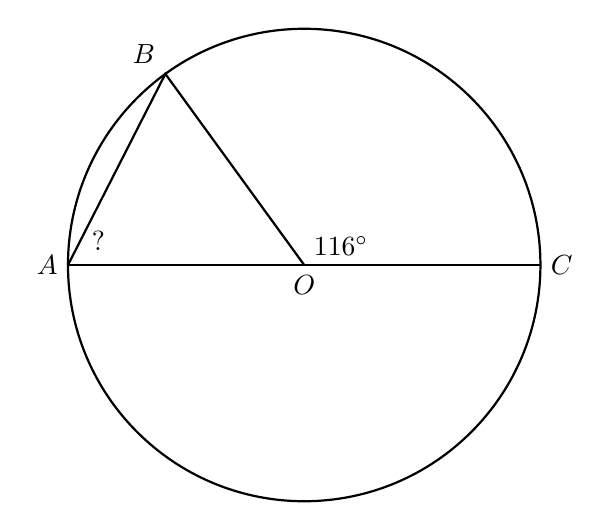
\begin{tikzpicture}[scale=0.6]
  \draw [thick] (0,0) circle [radius=5];
  \draw [-, thick] (-5,0) node[left]{$A$}--
  (0,0) node[below]{$O$}--
  (5,0) node[right]{$C$};
  \draw [-, thick] (0,0)--(126:5) node[above left]{$B$}--(-5,0);
  \node at (0, 0)[above right]{$116^\circ$};
  \node at (-4.7, 0.1)[above right]{?};
\end{tikzpicture}
\end{flushright} \vspace{2cm}

\item The triangle $ABC$, shown below, undergoes two rigid motions carrying it onto triangle $XYZ$. State the two isometric transformations. (be specific)
\begin{flushright}
  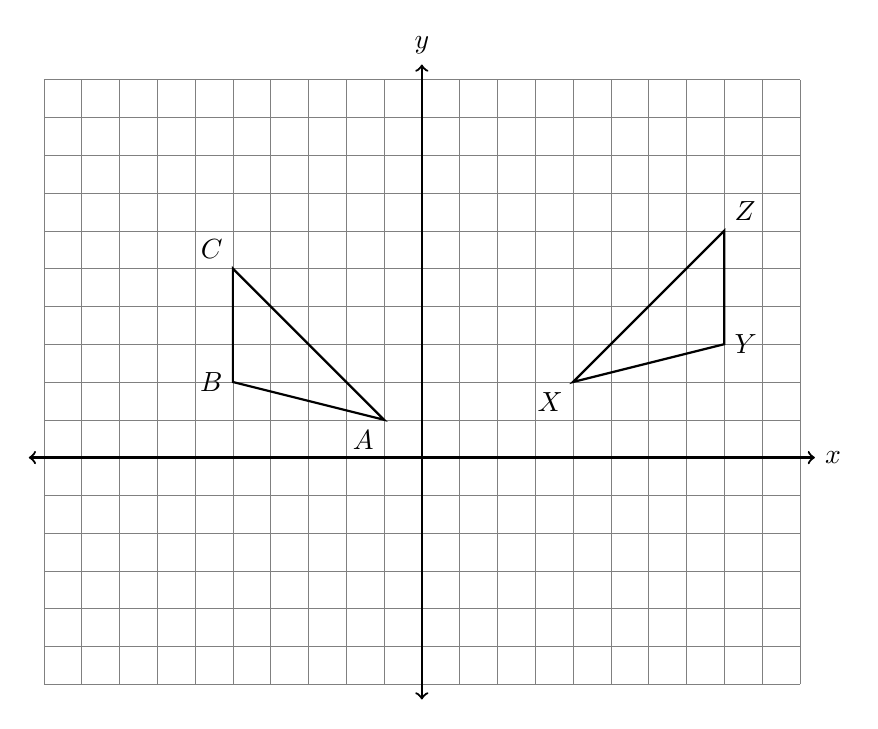
\begin{tikzpicture}[scale=.48]
    \draw [help lines] (-10,-6) grid (10,10);
    \draw [thick, <->] (-10.4,0) -- (10.4,0) node [right] {$x$};
    \draw [thick, <->] (0,-6.4)--(0,10.4) node [above] {$y$};
    \draw [thick]
      (4,2) node[below left] {$X$}--
      (8,3) node[right] {$Y$}--
      (8,6) node[above right] {$Z$}--cycle;
    \draw [thick]
      (-1,1) node[below left] {$A$}--
      (-5,2) node[left] {$B$}--
      (-5,5) node[above left] {$C$}--cycle;
  \end{tikzpicture}
\end{flushright}

\newpage
\item An angle bisector is shown below, with $\overrightarrow{AC}$ bisecting $\angle BAD$. Given $m\angle BAC = 6x+1$ and $m\angle BAD = 14x-15$, find $m\angle BAD$. (Show check)
\begin{flushright}
\begin{tikzpicture}[scale=0.7, rotate=30]
  \draw [<->, thick] (100:7)node[left]{$B$} 
  --(0,0)node[below]{$A$}
  --(6,0)node[below]{$D$}--(7,0);
  \draw [->, thick] (0,0)--(50:7)node[below right]{$C$};
  %\draw [fill] (0,0) circle [radius=0.05] node[below]{$A$};
  %\draw [fill] (5,0) circle [radius=0.05] node[below]{$B$};
\end{tikzpicture}
\end{flushright} \vspace{4cm}

\item Given parallel lines $\overleftrightarrow{AB} \parallel \overleftrightarrow{CDE}$ with $\overline{AC} \cong \overline{CD}$. If $m\angle BAD=68$ find $m\angle ACD$.
  \begin{flushright}
  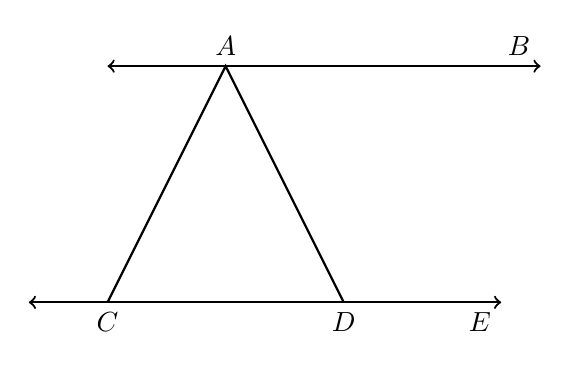
\begin{tikzpicture}
    \draw [<->, thick] (1,3)--(6.5,3) node[above left]{$B$};
    \draw [<->, thick] (0,0)--
      (5,0)--
      (6,0) node[below left]{$E$};
    \draw [-, thick] (1,0) node[below]{$C$}--
      (2.5,3) node[above]{$A$}--
      (4,0) node[below]{$D$};
  \end{tikzpicture}
  \end{flushright} \vspace{1.5cm}

\newpage
\item Of two supplementary angles, the measure of $\angle A$ is five times that of $\angle B$. Find $m\angle A$. \vspace{5cm} 

\item On the set of axes below, $\triangle ABC$ has vertices at $A(-2,0)$, $B(2,4)$, $C(4,-2)$, and $\triangle DEF$ has vertices at $D(4,0)$, $E(-4,8)$, $F(-8,-4)$.
\begin{center}
  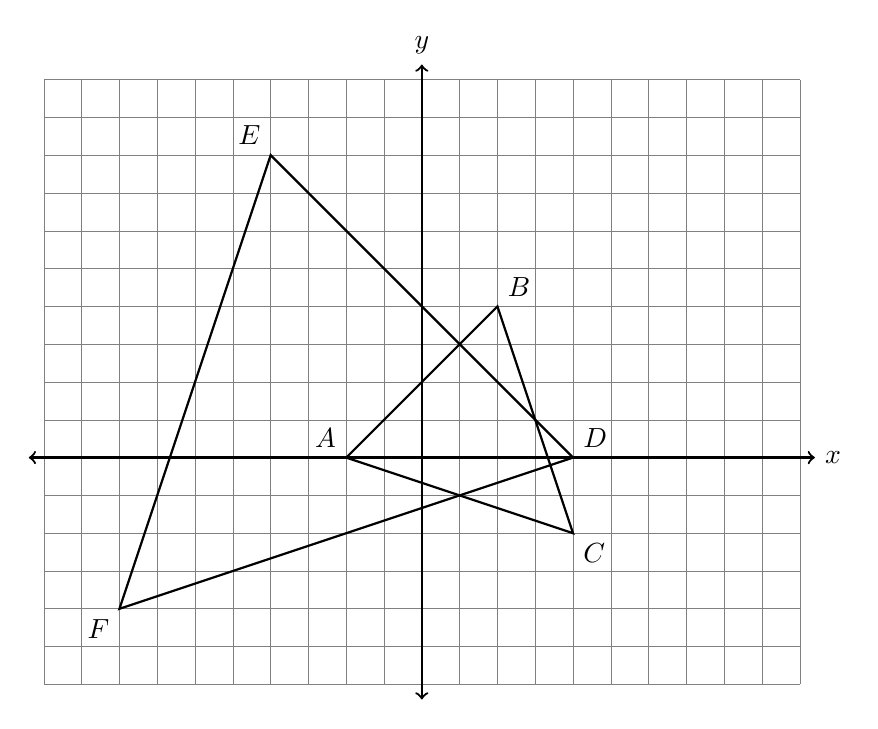
\begin{tikzpicture}[scale=.48]
    \draw [help lines] (-10,-6) grid (10,10);
    \draw [thick, <->] (-10.4,0) -- (10.4,0) node [right] {$x$};
    \draw [thick, <->] (0,-6.4)--(0,10.4) node [above] {$y$};
    \draw [thick]
      (-2,0) node[above left] {$A$}--
      (2,4) node[above right] {$B$}--
      (4,-2) node[below right] {$C$}--cycle;
    \draw [thick]
      (4,0) node[above right] {$D$}--
      (-4,8) node[above left] {$E$}--
      (-8,-4) node[below left] {$F$}--cycle;
  \end{tikzpicture}
\end{center}
Which tranformations map $\triangle ABC \rightarrow \triangle DEF$? Mark each statement True or False
  \begin{enumerate}
    \item A dilation with a scale factor of $-2$ centered at the origin \hfill True \quad False
    \item A dilation with a scale factor of $\frac{1}{2}$ centered at point $A$ \hfill True \quad False
    \item A dilation with a scale factor of 2 centered at the origin, followed by a rotation of $180^\circ$ about the origin \hfill True \quad False
    \item A dilation with a scale factor of 2 centered at the origin, followed by a reflection across the $y$-axis \hfill True \quad False
  \end{enumerate}

\newpage 
\item Triangle $ADE$ and its midline $\overline{BC}$ are drawn, with $B$ the midpoint of $\overline{AD}$ and $C$ the midpoint of $\overline{AE}$. The two medians $\overline{AE}$ and $\overline{AE}$ are drawn, as shown, intersecting in point $F$, the centroid.\\[0.25cm]
$\triangle FCB \sim \triangle FDE$ with scale factor $k=2$. 
Given $BC=8$ and $BF=5$. \\[0.25cm] Find $DE$ and $FE$.
\begin{flushright}
    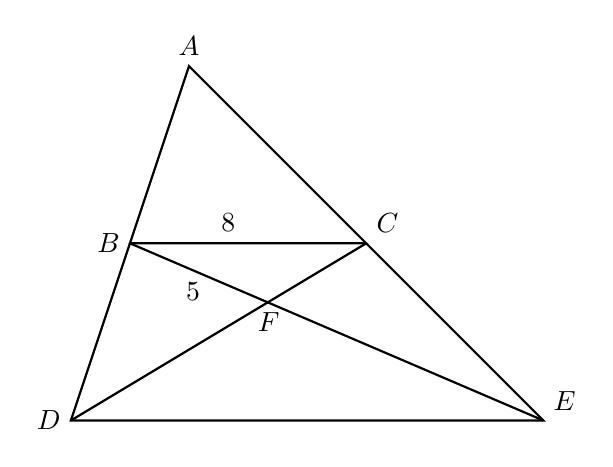
\begin{tikzpicture}[scale=0.5]
      \draw [thick]
      (0.5,1.5)node[left]{$B$}--
      (6.5,1.5)node[above right]{$C$}--
      (2,6)node[above]{$A$}--cycle;
      \draw [thick]
      (0.5,1.5)--
      (-1,-3)node[left]{$D$}--
      (11,-3)node[above right]{$E$}--(6.5,1.5);
      \draw [thick] (0.5,1.5)--(11,-3);
      \draw [thick] (6.5,1.5)--(-1,-3);
      \node at (3,2.5)[below]{$8$};
      \node at (3.5, -0.5)[right]{$F$};
      \node at (2.1, -0.2)[above]{$5$};
      %\node at (-0.7, -1)[above]{$5$};
    \end{tikzpicture}
  \end{flushright}

\item In  $\triangle ABC$ shown below, side $\overline{AC}$ is extended to point $D$ with $m\angle DAB=(11x+12)^\circ$, $m\angle C=(3x+3)^\circ$, and $m\angle B=(9x+2)^\circ$. \\[0.25cm]
What is $m\angle BAC$?
\begin{flushright}
    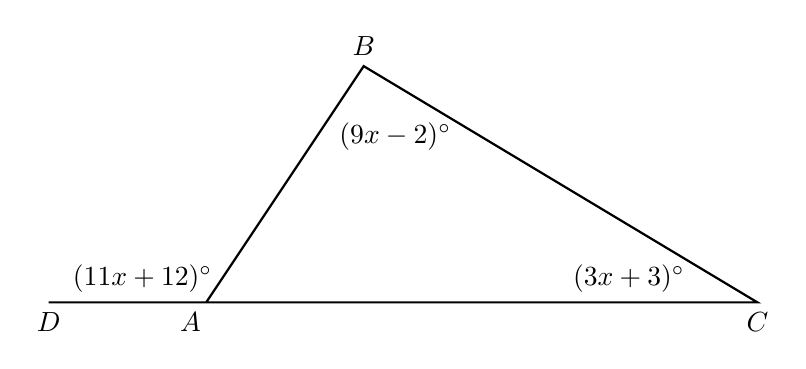
\begin{tikzpicture}
      \draw [thick](0,0)node[below]{$D$}--
        (1.8,0)node[below]{$A$}--
        (9,0)node[below]{$C$}--
        (4,3)node[above]{$B$} --(2,0);
        \node at (2.2,0)[above left]{$(11x+12)^\circ$};
        \node at (8.2,0)[above left]{$(3x+3)^\circ$};
        \node at (4.4,2.4)[below]{$(9x-2)^\circ$};
    \end{tikzpicture}
  \end{flushright}

\newpage
  \item Write down the slope perpendicular to the given slope.
  \begin{enumerate}
    \begin{multicols}{2}
    \item   $m= \frac{2}{3} \hspace{1cm} m_{\perp} = $ \vspace{1cm}
    \item   $m= -2 \hspace{1cm} m_{\perp} = $
    \item   $m= 0.25 \hspace{1cm} m_{\perp} = $ \vspace{1cm}
    \item   $m= -\frac{1}{5} \hspace{1cm} m_{\perp} = $
    \end{multicols}
  \end{enumerate} \vspace{1cm}

  
  \item The line $l$ has the equation $y=\frac{5}{2} x+9$.
  \begin{enumerate}
    \item What is the slope of the line $k$, given $k \parallel l$?
    \vspace{1.5cm}
    \item What is the slope of the line $j$, given $j \perp l$?
    \vspace{1.5cm}
  \end{enumerate}

  \item What is the slope of a line parallel to the line $2x+2y=14$?  \vspace{4cm}
  \item What is the slope of a line perpendicular to the line $-2x+y=1$?  
 
\newpage
  \item Note: The formula for distance is $\displaystyle d=\sqrt{(x_2-x_1)^2+(y_2-y_1)^2}$ \\[0.25in]
    Graph and label $\triangle ABC$ and find the lengths of its sides. $A(1,2)$, $B(9,8)$, $C(9,2)$.
    \begin{enumerate}
      \begin{multicols}{2}
      \item   $AC=$ \vspace{1.7cm}
      \item   $BC=$ \vspace{1.7cm}
      \item   $AB=$ \vspace{3cm}
        \begin{center}
          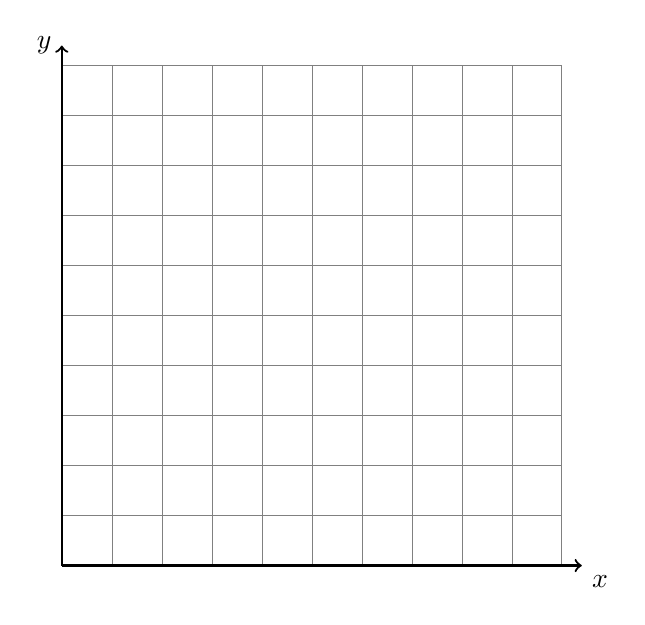
\begin{tikzpicture}[scale=.635]
            \draw [help lines] (0,0) grid (10,10);
            \draw [thick, ->] (0,0) -- (10.4,0) node [below right] {$x$};
            \draw [thick, ->] (0,0)--(0,10.4) node [left] {$y$};
          \end{tikzpicture}
          \end{center}
      \end{multicols}
    \end{enumerate}
    \vspace{1cm}

  \item Find $c$. \hspace{8cm}
    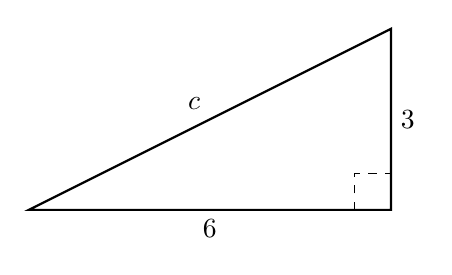
\begin{tikzpicture}[scale=1.15]
      \node at (2,1)[above left]{$c$};
      \node at (4,1)[right]{3};
      \node at (2,0)[below]{6};
      \draw [thick] (0, 0)--(4, 0)--(4, 2)--cycle;
      \draw [dashed] (4,0)++(-0.4,0)-- ++(0,0.4)-- +(0.4,0);
    \end{tikzpicture} \vspace{3cm}

  \item What is the length of $\overline{CD}$ if $C(3,-1)$ and $D(-2,11)$?

\newpage
  \item On the graph below, draw $\overline{AB}$, with $A(-2,3)$ and $B(5,1)$, labeling the end points. Determine and state the coordinates of the midpoint $M$ of $\overline{AB}$ and mark and label it on the graph.
  \begin{flushright}
    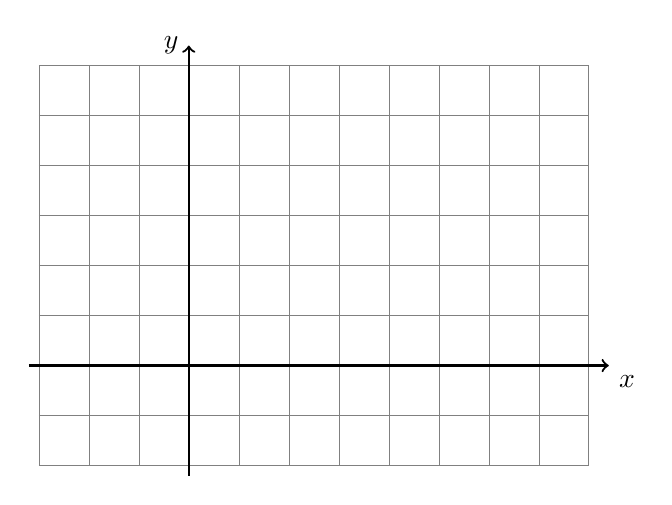
\begin{tikzpicture}[scale=.635]
      \draw [help lines] (-3,-2) grid (8,6);
      \draw [thick, ->] (-3.2,0) -- (8.4,0) node [below right] {$x$};
      \draw [thick, ->] (0,-2.2)--(0,6.4) node [left] {$y$};
    \end{tikzpicture}
  \end{flushright}
  \vspace{1cm}

  \item Spicy: On the set of axes below, graph the quadrilateral $ABCD$ having coordinates $A(-3,-3)$, $B(5,1)$, $C(6,8)$, and $D(-2,4)$. Find the slope of each of the four sides. What type of quadrilateral is $ABCD$? Justify your answer.
    \begin{flushright} %4 quadrant regents grid
      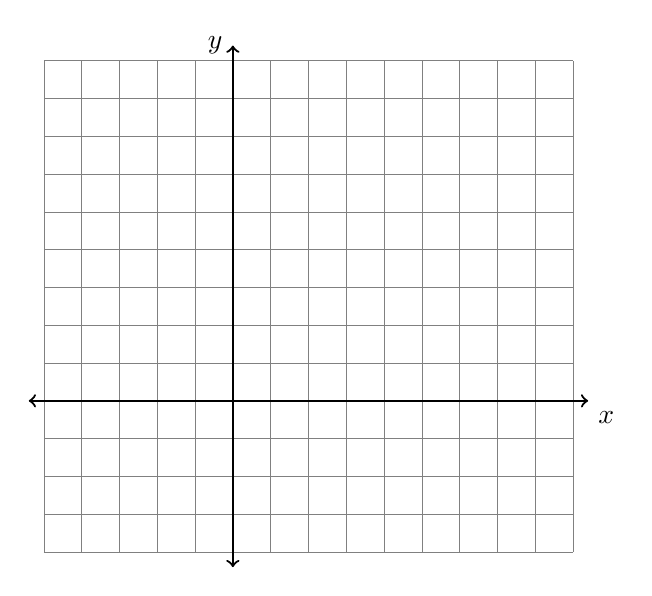
\begin{tikzpicture}[scale=.48]
        \draw [help lines] (-5,-4) grid (9,9);
        \draw [thick, <->] (-5.4,0) -- (9.4,0) node [below right] {$x$};
        \draw [thick, <->] (0,-4.4)--(0,9.4) node [left] {$y$};
        %\draw [thick] (-3,-3) node[below] {$A$}--
        %(5,1) node[right] {$B$}--
        %(6,8) node[right] {$C$}--
        %(-2,4) node[left] {$D$}--cycle;
        %\draw [fill] (5,0) circle [radius=0.1] node[above left] {$P$};
      \end{tikzpicture}
    \end{flushright}
    

\end{enumerate}
\end{document}

\item What is the midpoint of $\overline{HB}$, $H(80)$ and $B(120)$? \hspace{0.5cm}
  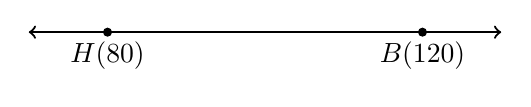
\begin{tikzpicture}[scale=1]
    \draw [thick, <->] (-1, 0)--(5,0);
    \draw [fill] (0,0) circle [radius=0.05] node[below]{$H(80)$};
    \draw [fill] (4,0) circle [radius=0.05] node[below]{$B(120)$};
  \end{tikzpicture} \vspace{1cm}

